\documentclass[tikz,border=8pt]{standalone}

\usepackage{xcolor}
\usepackage{tikz}

% -----------------------
% Color definitions
% -----------------------
\definecolor{varred}{RGB}{200,0,0}
\definecolor{aspectblue}{RGB}{0,70,160}
\definecolor{boxgray}{RGB}{245,245,245}

% NVIDIA green
\definecolor{nvidiagreen}{RGB}{118,185,0}

\begin{document}

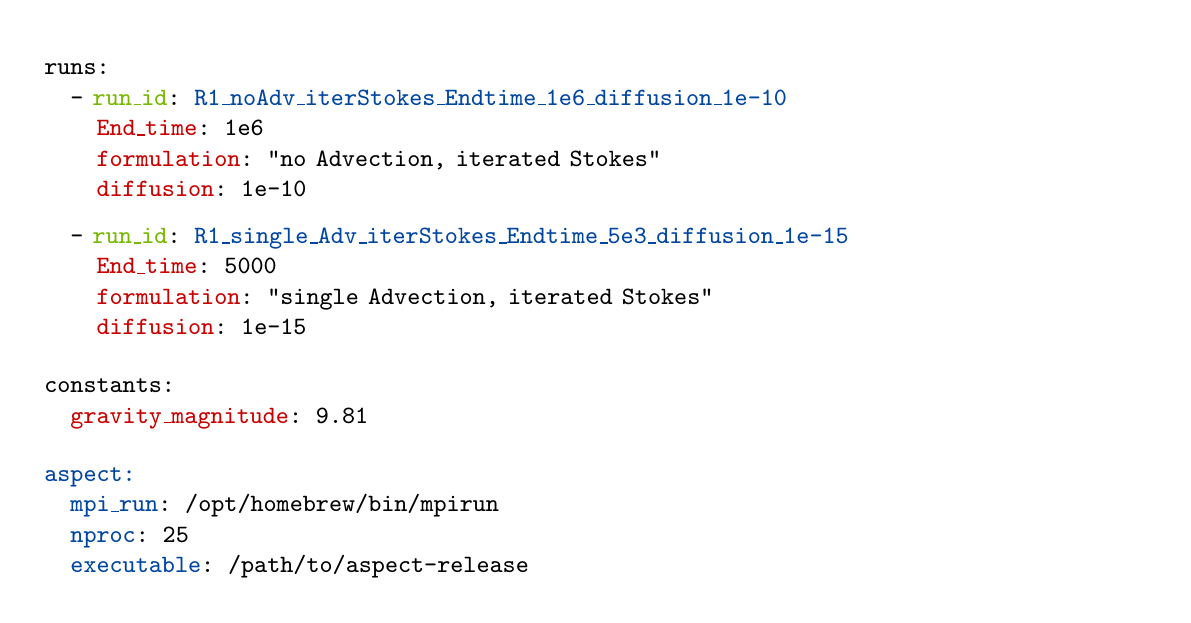
\begin{tikzpicture}

% \node[
%     draw,
%     rounded corners=6pt,
%     fill=boxgray,
%     inner sep=12pt,
%     text width=14cm
% ] (box)
\node[
    fill=white,
    inner sep=6pt,
    text width=14cm
] (box)
{
\ttfamily\small

\textbf{runs:}

\quad - \textcolor{nvidiagreen}{run\_id}: \textcolor{aspectblue}{R1\_noAdv\_iterStokes\_Endtime\_1e6\_diffusion\_1e-10} \\
\quad\quad \textcolor{varred}{End\_time}: 1e6 \\
\quad\quad \textcolor{varred}{formulation}: "no Advection, iterated Stokes" \\
\quad\quad \textcolor{varred}{diffusion}: 1e-10 \\[6pt]

\quad - \textcolor{nvidiagreen}{run\_id}: \textcolor{aspectblue}{R1\_single\_Adv\_iterStokes\_Endtime\_5e3\_diffusion\_1e-15} \\
\quad\quad \textcolor{varred}{End\_time}: 5000 \\
\quad\quad \textcolor{varred}{formulation}: "single Advection, iterated Stokes" \\
\quad\quad \textcolor{varred}{diffusion}: 1e-15 \\[10pt]

\textbf{constants:} \\
\quad \textcolor{varred}{gravity\_magnitude}: 9.81 \\[10pt]

\textcolor{aspectblue}{\textbf{aspect:}} \\
\quad \textcolor{aspectblue}{mpi\_run}: /opt/homebrew/bin/mpirun \\
\quad \textcolor{aspectblue}{nproc}: 25 \\
\quad \textcolor{aspectblue}{executable}: /path/to/aspect-release

};

\end{tikzpicture}

\end{document}